%DAN: compiled first time, so that's good!

\documentclass[letterpaper,11pt]{article}
\usepackage[left=2cm,top=2cm,right=2cm,bottom=1.5cm,head=.5cm,foot=.5cm]{geometry}
\usepackage{graphicx}
\usepackage{amsmath}
\usepackage{hyperref}
\usepackage{cite}
\usepackage{xr-hyper}
\usepackage{float}
\usepackage{xr} 
\usepackage{adjustbox}
\usepackage{url}
\usepackage{multirow}
\usepackage{longtable}
\usepackage{subfig}
\usepackage{float}
\usepackage{setspace}
\usepackage{lineno}
\usepackage{natbib}
\usepackage{amsmath}
\usepackage{authblk}
\usepackage{xr}
\usepackage{relsize}
\usepackage{tikz}


%%%% HELPER CODE FOR DEALING WITH EXTERNAL REFERENCES
% (from an answer by cyberSingularity at http://tex.stackexchange.com/a/69832/226)
%%%

\usepackage{xcite}

\usepackage{xr}
\makeatletter
\newcommand*{\addFileDependency}[1]{% argument=file name and extension
  \typeout{(#1)}% latexmk will find this if $recorder=0 (however, in that case, it will ignore #1 if it is a .aux or .pdf file etc and it exists! if it doesn't exist, it will appear in the list of dependents regardless)
  \@addtofilelist{#1}% if you want it to appear in \listfiles, not really necessary and latexmk doesn't use this
  \IfFileExists{#1}{}{\typeout{No file #1.}}% latexmk will find this message if #1 doesn't exist (yet)
}
\makeatother

\newcommand*{\myexternaldocument}[1]{%
    \externaldocument{#1}%
    \addFileDependency{#1.tex}%
    \addFileDependency{#1.aux}%
}
%%% END HELPER CODE

% put all the external documents here!
\myexternaldocument{SI}

\title{Toy Workflow}
\author[a,*]{Nilanjan}

\affil[a]{Department of Molecular Biosciences, University of Kansas}
\affil[*]{Corresponding author, nilanjan.roy@ku.edu}

\begin{document}

\maketitle

\section{Introduction}
This is a toy analysis following the workflow learned in class.

\section{Methods}
The analysis used a linear model to fit data from a simple dataset.

\subsection{Equation}
The model fits the following equation:
\begin{equation}
y = \beta_0 + \beta_1 x
\label{eq:linear_model}
\end{equation}

\section{Results}
Figure~\ref{fig:plot} shows the relationship between \(x\) and \(y\).

\begin{figure}[H]
    \centering
    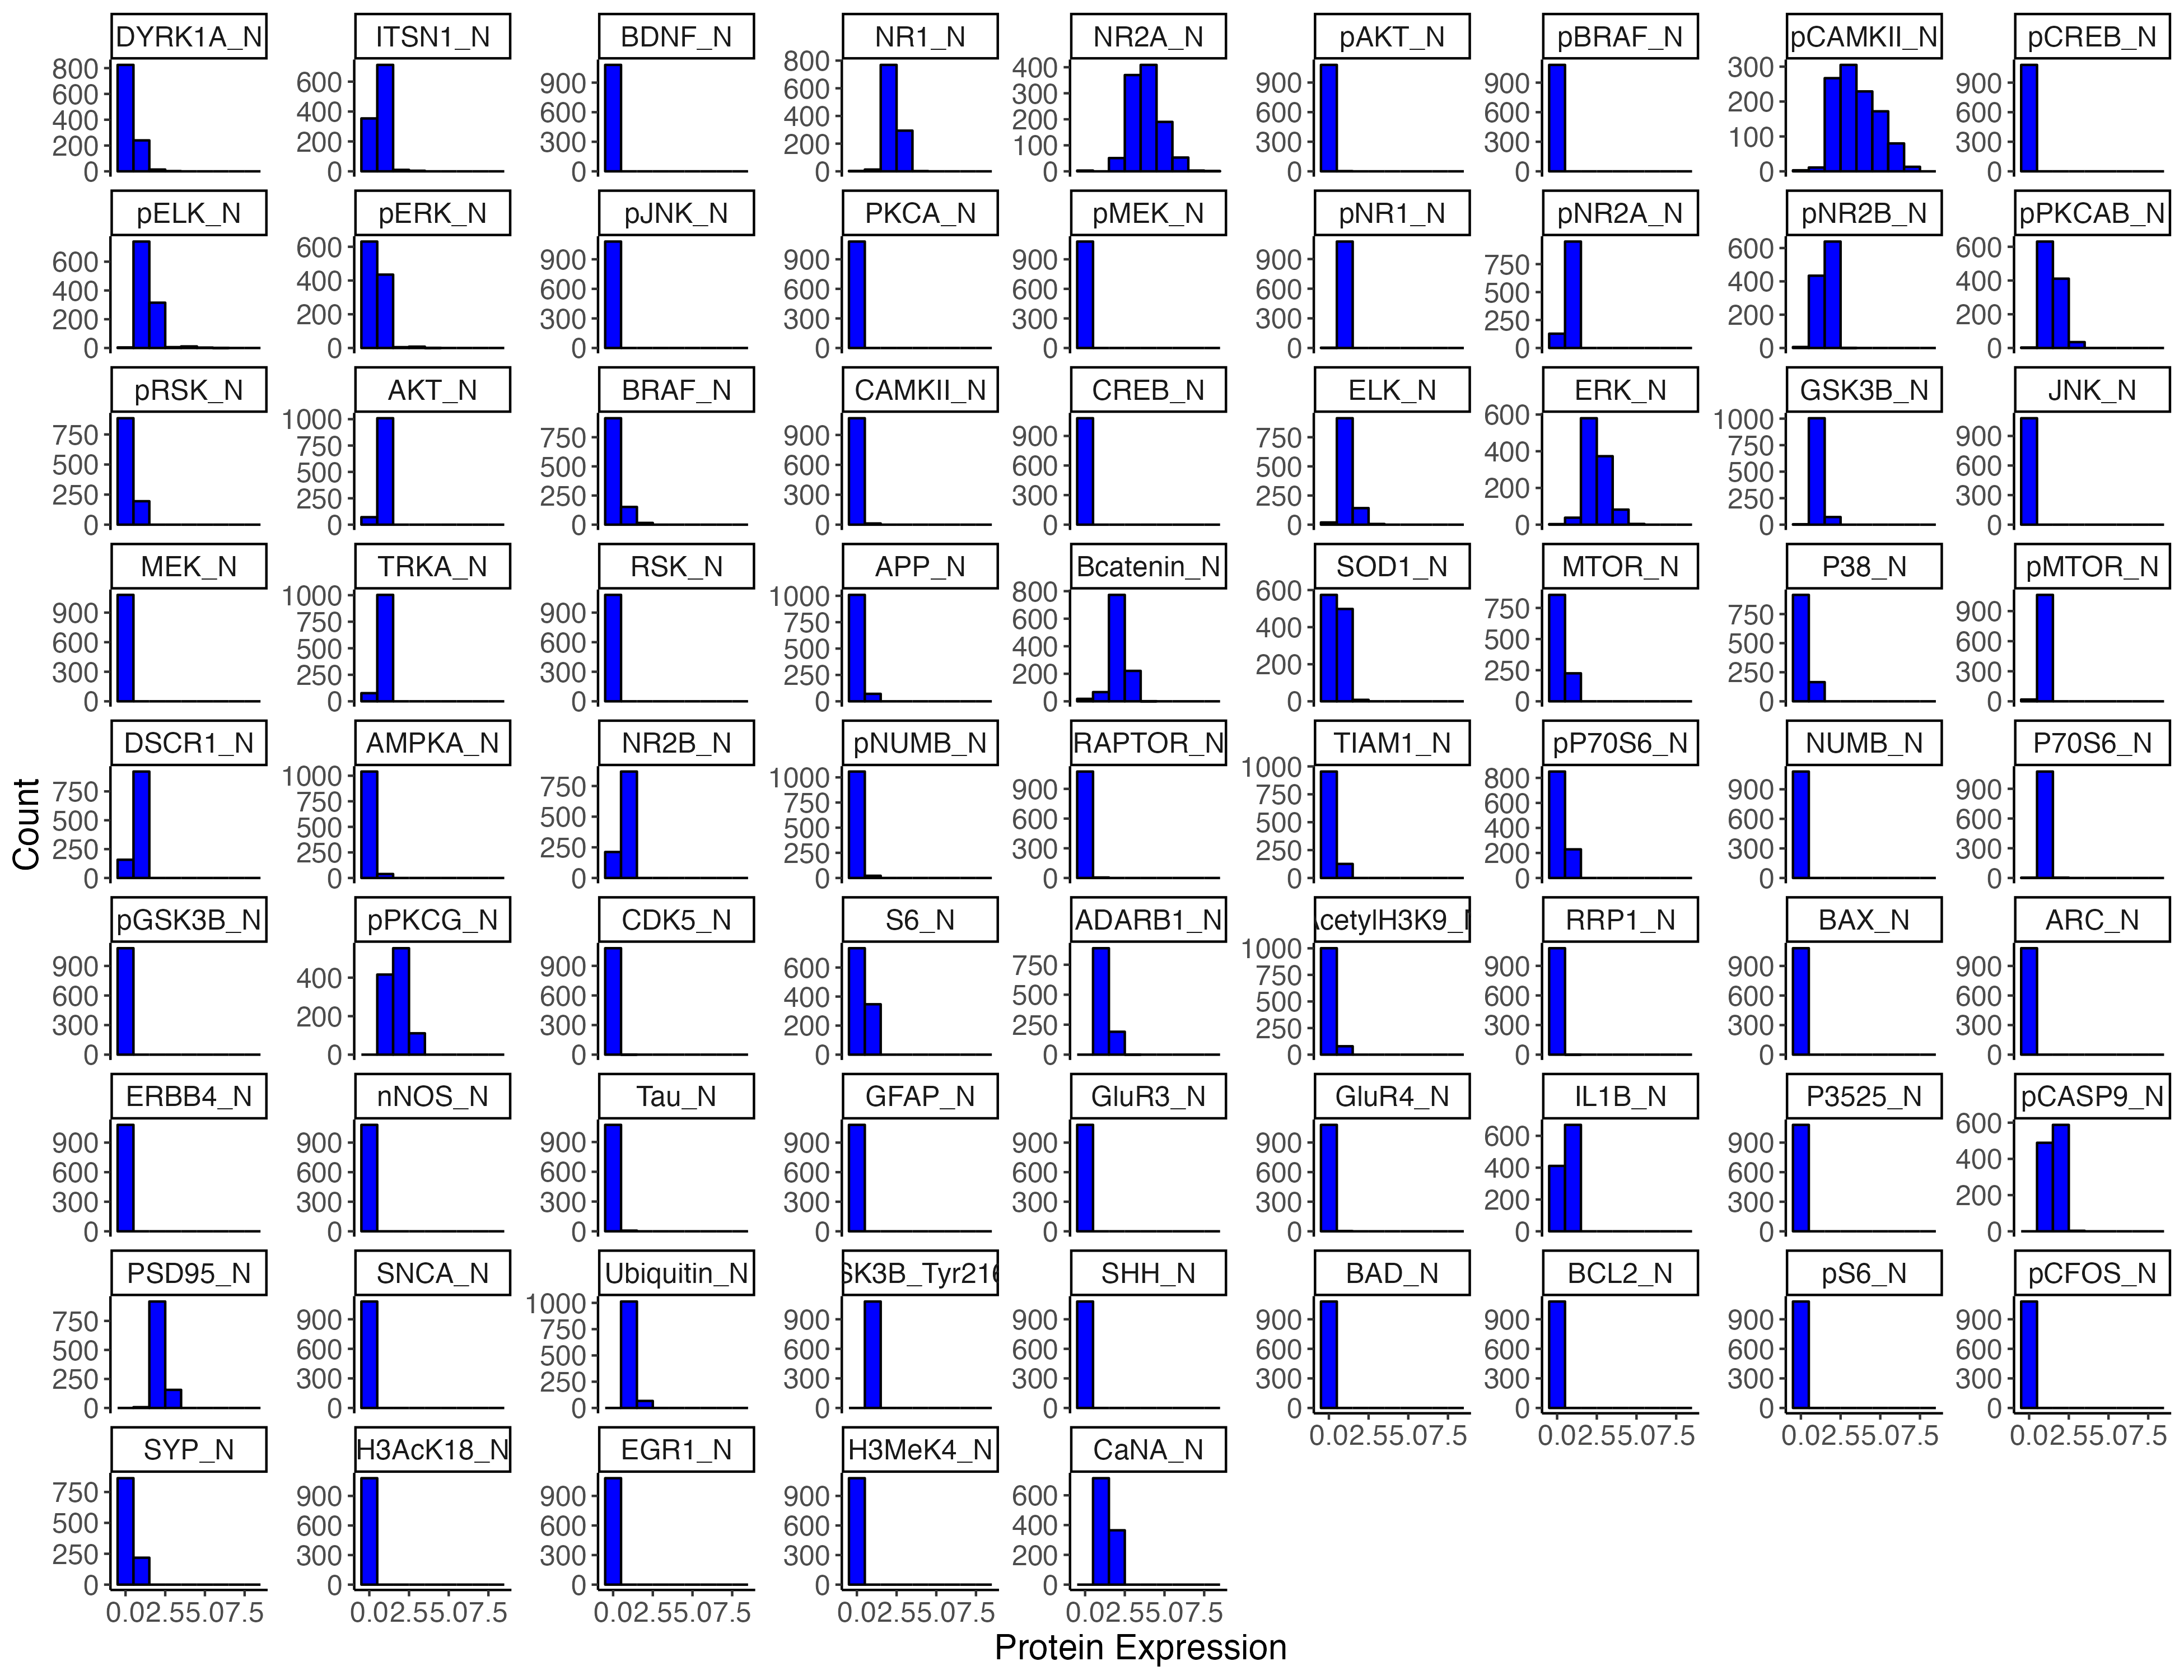
\includegraphics[width=0.5\textwidth]{Results/protein_expression_histograms.png}
    \caption{Histogram of protein expression levels.}
    \label{fig:plot}
\end{figure}

In this study, we build upon findings detailed in Section~\ref{sec:method_details} of the SI. The equation reference is Eq.~\ref{eq:linear_model}. This is a reference ~\cite{example2023}. Example table is below.

\begin{table}[ht]
\centering
\begin{adjustbox}{width=\textwidth}
\begin{tabular}{lrrrrrrrrrr}
  \hline
 & \multicolumn{1}{c}{DYRK1A\_N} & \multicolumn{1}{c}{ITSN1\_N} & \multicolumn{1}{c}{BDNF\_N} & \multicolumn{1}{c}{NR1\_N} & \multicolumn{1}{c}{NR2A\_N} & \multicolumn{1}{c}{pAKT\_N} & \multicolumn{1}{c}{pBRAF\_N} & \multicolumn{1}{c}{pCAMKII\_N} & \multicolumn{1}{c}{pCREB\_N} & \multicolumn{1}{c}{pELK\_N} \\ 
  \hline
DYRK1A\_N & 1.00 & 0.96 & 0.37 & 0.31 & 0.34 & -0.15 & -0.06 & -0.16 & 0.07 & 0.79 \\ 
ITSN1\_N & 0.96 & 1.00 & 0.47 & 0.44 & 0.44 & -0.10 & -0.03 & -0.11 & 0.20 & 0.79 \\ 
BDNF\_N & 0.37 & 0.47 & 1.00 & 0.83 & 0.76 & 0.38 & 0.46 & 0.28 & 0.65 & 0.47 \\ 
NR1\_N & 0.31 & 0.44 & 0.83 & 1.00 & 0.88 & 0.28 & 0.33 & 0.33 & 0.64 & 0.44 \\ 
NR2A\_N & 0.34 & 0.44 & 0.76 & 0.88 & 1.00 & 0.16 & 0.17 & 0.30 & 0.43 & 0.43 \\ 
pAKT\_N & -0.15 & -0.10 & 0.38 & 0.28 & 0.16 & 1.00 & 0.84 & 0.47 & 0.63 & 0.08 \\ 
pBRAF\_N & -0.06 & -0.03 & 0.46 & 0.33 & 0.17 & 0.84 & 1.00 & 0.39 & 0.63 & 0.16 \\ 
pCAMKII\_N & -0.16 & -0.11 & 0.28 & 0.33 & 0.30 & 0.47 & 0.39 & 1.00 & 0.42 & -0.06 \\ 
pCREB\_N & 0.07 & 0.20 & 0.65 & 0.64 & 0.43 & 0.63 & 0.63 & 0.42 & 1.00 & 0.25 \\ 
pELK\_N & 0.79 & 0.79 & 0.47 & 0.44 & 0.43 & 0.08 & 0.16 & -0.06 & 0.25 & 1.00 \\ 
  \hline
\end{tabular}
\end{adjustbox}
\caption{Correlation coefficients between different proteins.}
\label{tab:protein_correlations}
\end{table}



\section{Discussion}
This simplified workflow demonstrates the application of R and LaTeX in scientific analysis.

\bibliographystyle{plain}
\bibliography{references}

\end{document}
